\documentclass[9pt,conference,a4paper]{IEEEtran}
\IEEEoverridecommandlockouts

%\usepackage{...}
\usepackage{mathpazo}
\usepackage[T1]{fontenc}
\usepackage[latin9]{inputenc}
%\usepackage[letterpaper]{geometry}
%\geometry{verbose,tmargin=0.15\paperwidth,bmargin=0.15\paperwidth,lmargin=0.2\paperwidth,rmargin=0.15\paperwidth}
\usepackage{bm}
\usepackage{amsmath}
\usepackage{graphicx}
\usepackage{setspace}
\usepackage{amssymb}
\usepackage{esint}
\usepackage[british,english]{babel}

\title{Cartesian grid q-space reconstruction}
\author{
	\IEEEauthorblockN{
		Eleftherios Garyfallidis\IEEEauthorrefmark{1} and
		Ian Nimmo-Smith\IEEEauthorrefmark{2}
	}

	\IEEEauthorblockA{\IEEEauthorrefmark{1} University of Cambridge}
	\IEEEauthorblockA{\IEEEauthorrefmark{2} MRC Cognition and Brain Sciences Unit}

%	\thanks{This work is supported by ...}
}

\begin{document}
\maketitle

% \makeatletter
% \numberwithin{figure}{section}
% \numberwithin{table}{section}
% \makeatother

%\section*{Cartesian Grid Q-space Reconstruction}


%\section*{Overview}

% Between one to two thirds of imaging voxels in the human brain's white
% matter are thought to contain multiple fiber crossings~\cite{Behrens2007NeuroImage},
% in which case the Diffusion Tensor model proposed by Basser et al.~\cite{Basser1994}
% breaks down. High Angular Resolution Diffusion Imaging (HARDI) methods
% \cite{Tuch2002} such as Diffusion Spectrum Imaging (DSI) \cite{callaghan1988nmr},
% \cite{wedeen2005mapping} or Higher Order Tensors \cite{ozarslan2003generalized},
% \cite{barmpoutis2009regularized} and many more reconstruction methods
% have been proposed to overcome the limitations of the Diffusion Tensor.
% Although all methods have some underlying assumptions; we generally
% separate them in two categories a) model-based and b) model-free.
For the purpose of the HARDI reconstruction workshop we used GQI2
\cite{Yeh2010}, \cite{Garyfallidis_thesis} a non-parametric method to
find the ODFs \cite{Tuch2002}, \cite{aganj2010reconstruction} for dMRI
acquisitions on a keyhole cartesian grid in
$q$-space\,\cite{Tuch2002}. From these ODFs we find the number of peaks
(number of fiber compartments); if this number equals 1, we report the ODF from
fitting the Single Tensor to the data, otherwise we report the original
GQI2 ODF.


%\section{Theory}

% According to \cite{Callaghan1991OUP}, \cite{callaghan1988nmr} using
% the narrow pulse gradient spin echo (PGSE) sequence of Tanner and
% Stejskal. The \textbf{k}-space reconstruction gives us diffusion weighted
% image data $S$ which reveal the average propagator $P_{\Delta}$
% of each voxel according to the following equation \begin{eqnarray}
% S(\mathbf{v},\mathbf{q}) & = & \int\rho(\mathbf{v})P_{\Delta}(\mathbf{v},\mathbf{r})\exp(i2\pi\mathbf{q}\cdot\mathbf{r})d\mathbf{r}.\label{eq:W}\end{eqnarray}


% \noindent where$\Delta$ is the time between diffusion gradients,
% $P_{\Delta}$ is the average diffusion propagator (transition probability
% distribution), \textbf{$\mathbf{v}$} is the voxel coordinate, and
% $\mathbf{r}$ is the diffusion displacement. For the rest of the chapter
% we consider each voxel independently and assume intra-voxel spatial
% homogeneity so we can drop explicit reference to $\mathbf{v}$and
% $\Delta$. We can also replace the spin density \foreignlanguage{british}{$\rho(\mathbf{v})$}
% with $S_{0}$ i.e. the measured signal without diffusion weighting
% $\mathbf{q}=\mathbf{0}$. Therefore we can write\begin{eqnarray}
% S(\mathbf{q}) & = & S_{0}\int P(\mathbf{r})\exp(i2\pi\mathbf{q}\cdot\mathbf{r})d\mathbf{r}\label{eq:S}\end{eqnarray}


% By applying the 3D Fourier transform in eq. \ref{eq:S} we can reconstruct
% the average propagator also known as the diffusion spectrum \cite{WWS+08}\begin{eqnarray}
% P(\mathbf{r}) & = & S_{0}^{-1}\int S(\mathbf{q})\exp(-i2\pi\mathbf{q}\cdot\mathbf{r})d\mathbf{r}\label{eq:P}\end{eqnarray}
% \noindent or diffusion propagator. 

% Following the approach of Wedeen et al.
% \cite{Wedeen} 
% %that the dMRI signal is positive for any type of spin
% %motion without net flux (i.e.~spin displacements due to thermal molecular
% %agitation) or other random fluxes such as intravoxel incoherent motion.
% we relate the diffusion displacement propagator to the modulus of the complex RF signal $S$ 
% by
% \begin{eqnarray}
% P(\mathbf{r}) & = & S_{0}^{-1}\int|S(\mathbf{q})|\exp(-i2\pi\mathbf{q}\cdot\mathbf{r})d\mathbf{r}\label{eq:P_modulus}
% \end{eqnarray}

% The modulus of the signal coincides with the output of the standard
% MRI scanners as dMRI and that simplifies the acquisition procedure.
% Since we are mainly interested in the directional structure of the underlying
% tissue, we further simplify the data by taking the weighted radial
% summation of $P(\mathbf{r})$
% \begin{equation}
% \psi_{DSI}(\hat{\mathbf{u}})=\int_{0}^{\infty}P(r\hat{\mathbf{u}})r^{2}dr\label{eq:ODF_DSI}
% \end{equation}
% This defines the orientation density function (ODF) for DSI which
% measures the quantity of diffusion in the direction of the unit vector
% $\mathbf{\hat{u}}$ where $\mathbf{r=}r\hat{\mathbf{u}}$.

Following the approach of Wedeen et al.~\cite{WWS+08} 
the ODF can be derived by obtaining the diffusion propagator from the dMRI signal
by a Fourier transform on the cartesian lattice  $P(\mathbf{r})=\mathcal{F}(S_0^{-1}S(\mathbf{q}))$ and then integrating radially. 
\begin{equation}
\psi_{DSI}(\hat{\mathbf{u}})=\int_{0}^{\infty}P(r\hat{\mathbf{u}})r^{2}dr\label{eq:ODF_DSI}
\end{equation}
Yeh
et al.~\cite{Yeh2010} proposed a direct way to calculate a slightly
different ODF using the Cosine transform. 
They estimated the spin density weighted propagator $Q$ via
from an unweighted truncated radial projection
\begin{eqnarray}
\psi_{GQI}(\mathbf{\hat{u}}) & = & \intop_{0}^{\lambda}Q(r\mathbf{\hat{u}})dr\label{eq:SDF}\nonumber\\
 & = & \lambda\int S(\mathbf{q})\mathtt{sinc}(2\pi r\mathbf{q}\cdot\mathbf{\hat{u}})d\mathbf{q}
\end{eqnarray}
where $\lambda$ is a smoothing factor called the diffusion sampling length.

We have instead developed an ODF like the one produced using
DSI where we need to take into consideration the weighted truncated
radial projection $r^2$. This will give us a different ODF which we symbolize
with $\psi_{GQI2}$\begin{eqnarray}
\psi_{GQI2}(\mathbf{\hat{u}}) & = & \intop_{0}^{\lambda}Q(r\mathbf{\hat{u}})r^{2}dr\nonumber\label{eq:SDF2}\\
 & = & \lambda^{3}\int S(\mathbf{q})H(2\pi r\mathbf{q}\cdot\mathbf{\hat{u}})d\mathbf{q}\end{eqnarray}
\noindent where $H(x)=\begin{cases}
\frac{2\cos(x)}{x^{2}} & +\frac{(x^{2}-2)\sin(x)}{x^{3}},x\neq0\\
 & 1/3\qquad\qquad,x=0\end{cases}$.
\begin{flushleft}
This equation can be implemented analytically in a simple matrix form
\begin{eqnarray}
\bm{\psi}_{GQI2} & = & \mathbf{s}\cdot\mathtt{H}((6D.G\circ\mathbf{b}\circ\mathbb{1})\cdot G)\lambda^{3}/\pi\label{eq:GQI2}
\end{eqnarray}

\par\end{flushleft}

\begin{flushleft}
where $\cdot$ denotes standard matrix or vector dot product, $\circ$
denotes the Hadamard product,  $\bm{\psi}_{GQI}$ as a
MD vector with components corresponding to the selected
directions $\hat{\mathbf{u}}$ on the ODF sphere, $\mathbf{s}$ is
a vector with all the signal values, $D=0.0025$
where $D$ is the free water diffusion coefficient,
$G$ is the $N\times3$ matrix with the gradient vectors, $\mathbf{b}$
is the $N\times1$ matrix with the b-values and $\mathbb{1}$ is the
$N\times3$ incidence matrix where all values are equal to $1$.
\par\end{flushleft}

We use $\lambda=3.0, 3.3, 3.5$ with the provided phantom data with SNRs $10, 20, 30$
respectively. In the case where a single peak is found the Single
Tensor model is fitted using Weighted Least Squares and the standard
ODF for that is generated. 


%\section*{Conclusion}

% Non-parametric methods have the advantage of representing the signal
% with minimum number of assumptions and without needing any fitting.
% For many years there has been a trend in science to prefer model-based
% rather than model free (non-parametric) methods. This is perhaps because
% model-based can be easier to describe, and more readily allow the
% use of popular Bayesian approaches. However, there are some crucial
% issues with fitting: (a) Usually the interesting models have many
% parameters and that makes fitting very slow. (b) Commonly non-linear
% fitting is needed and accurate fitting is not trivial. (c) Often the
% model does not represent precisely the complexity of the real problem.
% (d) The more complex the model, the more difficult to fit \cite{rice2006mathematical},
% \cite{lee1997bayesian}, \cite{montgomery2001introduction}. 
The source code for the methods described here can be found in DIPY
(dipy.org).  An example of our method can be seen in Fig.~1.  GQI2 is a
method theoretically identical with the framework of Equatorial
Inversion Transform (EIT) \cite{Garyfallidis_thesis} with Laplacian
weighting. This builds on the formulation in eq.~\ref{eq:GQI2}.

\noindent~Model-based methods for ODF estimation, like the Single Tensor
or Multi Tensor, require a number of parameters to be fitted. By
contrast for model-free methods fitting is not necessary and the
directionality of the underlying tissue can be approximated by a
re-parametrization or re-transformation of the signal. The latter is
usually more efficient than fitting models with many parameters which
typically call for iterative methods.

%
\begin{figure}
\begin{centering}
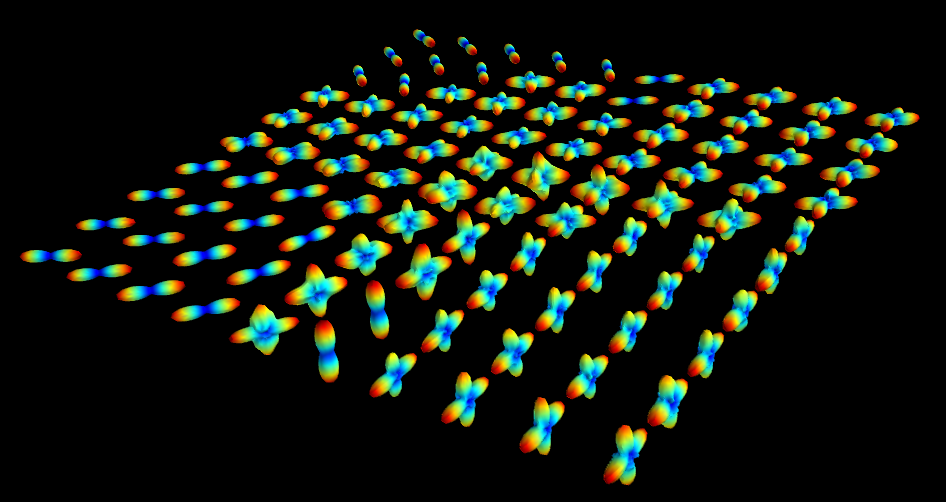
\includegraphics{hardi_isbi2012/isbi2012}
\end{centering}
\caption{Result showing our reconstruction ODFs with the training data set
(SNR 30) provided by the organizers of the HARDI Workshop 2012}
\end{figure}


\selectlanguage{british}%
\bibliographystyle{ieeetr}
\bibliography{diffusion}
\selectlanguage{english}

%\begin{thebibliography}{}
%\bibitem{einstein94}A. Einstein, A. Einstein and A. Einstein, ``Title'', Journal, Vol, page (year).
%\end{thebibliography}

\end{document}
